\chapter{Background}
% "Ongelmakentän esittely".

On this chapter the three prime themes around this thesis are introduced. Basic knowledge of these themes are required in order to fully comprehend all the aspects on the case study investigated on this thesis later on. 

The basics of \textit{web as an application platform} and more precisely the \textit{single-page application} paradigm is introduced as it is the method how the web application is built on the case study. The concept of \textit{computer supported collaborative work} is introduced since the case study's application is essentially that: multiple users collaboratively viewing and editing the same data set. The most usual types of \textit{connectivity issues} and the reasons for them are portrayed, since the disruption created by them to the case study's application created the actual need for offline supported functionalities in the first place. 




%% ----------------------------------
\section{Web Applications}

In the past decade the software industry as a whole has been facing a major paradigm shift on the way how and where applications are developed and operated. Progress in web technologies and standards have made possible for the browser environment to be a more and more powerful but still universal computing platform. Software applications that were previously build for different kind of operating system and CPU combinations are now written with web technologies and ran on the browser. This change is mainly accomplished by the power of distribution the web platform provides. Software provider or the organization's IT function does not have to take care of updating end user software to the latest version anymore, because the client-server paradigm\cite{berson_client-server_1992} makes running outdated software version virtually impossible. In a traditional desktop application patching the software to fix bugs or introducing a new feature requires downloading a installer or a patcher and then it must be ran on the computer. This requires action from the user or from the IT function. This might not cover the whole upgrading process in every situation: sometimes updating dependent libraries or operating system might be required. It also enables possibility for different computers to be running different versions of the software, creating circumstances for version mismatches between different clients. \cite{jazayeri_trends_????} \cite{taivalsaari_mashware:_2009} %[jazayeri 3.3] [taivalsaari_mashware:_2009]

The move from individual installations to a centralized reverses the general model how software is operated since the start of the personal computing revolution \cite[Chapter 3.3]{jazayeri_trends_????}. As stated above, this comes with many benefits. One of the most important ones is the (almost) unified platform provided for the developers. Thanks to automatic update mechanisms of the modern browsers, this platform is one of the fastest updating ones there is when it comes to speed of patches applied to end users' computers \cite{duebendorfer_why_2009}. Due to the easiness of the deployment process, it is not unusual to see web application rolling in releases to production on daily or even on hourly basis \cite[Chapter 3.3]{jazayeri_trends_????}.



% ###
\subsection{Single-Page Applications}
\label{subsec:spa}
% - yleisesti tuotantojavaskriptistä, yks yhdistetty&minimifoitu .js-möykky tuotannossa (tähän viittaan implementaatio-osuudessa)?
% - AMD-moduulin avaus?


Executing complicated applications on the web platform has been made possible by the evolution of the web pages from ``classic'', static presentation consisting of single pages to a more interactive and collaborative web applications. On the early phases of World Wide Web user navigated through hyperlinks within single pages each of them being formed and served by the server. Client, the browser, was responsible only for rendering the response of the server. \cite{taivalsaari_mashware:_2009} The current state of technology allows more of the functionality to be moved or duplicated from the server to the client. When before web pages on the browser were stateless, and the state transforms were done while moving to a new page, now it is possible for the browser to handle the state transitions and retrieve only the needed data from the server when required via AJAX\footnote{Asynchronous JavaScript + XML}-requests. \cite{paulson_building_2005}

The applications following the paradigm described above can be generalized to be \textit{single-page applications}. These kind of web applications makes a request to the server, and based on the data of the server's response, they form the layout of the page manipulating the browser's \textit{Document Object Model} in real time. This is contrary to the traditional paradigm where based on the client's request the server creates the layout for the data and sends an whole HTML page as a response, and the whole page is refreshed in result. This is also the etymology behind the name of the paradigm: there is no need for user to navigate away from the page, even when the views on the application change.

The application state handling on the browser environment and the increased amount of possibilities on the browser creates the basis for modern web development and the platform for the offline feature: the single-page application. Single-page application is tightly relevant to other hype terms such as \textit{Web 2.0} and the nowadays partly old-fashioned term \textit{DHTML}\footnote{Dynamic HTML}. All single-page applications could be called Web 2.0 applications, but not all Web 2.0 applications are single-page applications. Whereas traditional web pages where synchronously fetched and generated by the web server, single-page application relies on asynchronous pattern on data fetching. \cite{garrett_ajax:_2005} With the asynchronous pattern the browser can fetch resources on smaller chunks when the need arises, usually through REST APIs \cite{masse_rest_2011}. This also makes possible the premise for an \textit{occasionally connected application}, meaning that the web application can function without having a continuous Internet connection \cite{casario_html5_2011}. The application has the ability to fetch data from the API when there is connectivity, and when the connectivity disappears it can function with application logic downloaded to the browser.  This widens a lot the range of use cases which can be covered by web applications.



% ###
\subsection{REST APIs}
% - JSON -termin avaus?
% - REST API:sta jotain (Päikky cachettaa nimenomaan tämäntyyppisiä requesteja)\citation{taivalsaari_mashware:_2009}
% - kuva havainnollistamaan että SPA hakee resursseja yksitellen ja vanhassa mallissa haetaan kokonaisia sivuja?
% - tarviikohan AJAXista tänne jotain?

REST is a term first time introduced by \textit{Roy Fielding} in his Ph.D. dissertation \cite{fielding_architectural_2000} as an description for an architecture style of networked systems. The REST acronym stands for \textit{Representational State Transfer}. Even the term REST comes up often in materials relating web technologies, it has to be remembered that it is more of an idea for architectural style than an actual well-defined standard. 

Roy Fielding explained the term on his dissertation in the following way:
\begin{quote}
	``Representational State Transfer is intended to evoke an image of how a well-designed Web application behaves: a network of web pages (a virtual state-machine), where the user progresses through an application by selecting links (state transitions) resulting in the next page (representing the next state of the application) being transferred to the user and rendered for their use.''
\end{quote}

The momentum behind the wide use of the REST principles rises from the key motivation behind it: REST captures the key components and ideas of which made the Web successful. These characteristics are in use with guiding the evolution of the Web today. \cite{costello_building_2007}

\begin{figure}[t]
\begin{center}
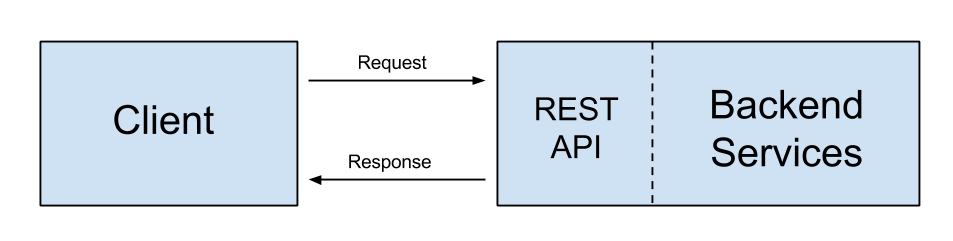
\includegraphics[width=0.8\textwidth]{assets/restapi.png}
\end{center}
\caption{Basic structure of a REST API service}
\label{fig:restapi}
\end{figure}

All the single-page applications that interact with data that is used by various clients requires some kind of backend service. Usually this is provided by creating \textit{application programming interfaces} (later on referrenced by APIs) on the backend for the client-server communication. In practice API exposes methods for fetching and altering the server's data. Therefore APIs can be thought as the \textit{face} for the web service, aimed for listening and responding the clients' requests. \cite{masse_rest_2011}

In the Figure~\ref{fig:restapi} can be seen a retold presentation from Masse (2011) about the general principle regarding a REST API. Well designed REST API is easily understood by humans, since the URLs themselves should describe precisely what resources will be returned to requests send to them. A REST API can be thought as an assembly of interlinked resources. This resources forms the REST API's \textit{resource model}. \cite{masse_rest_2011}

REST APIs plays an integral part on the single-page applications. Basically after the client side code is initialized on the browser, all the actual content (depending on the context whatever that might be) is fetched to the browser via an API which nowadays are almost always RESTful. All the modification and the creation of the data is also done through the functionality exposed to the client by the API. Usually the data is transferred between the client and the server using \textit{JSON objects} (JavaScript Object Notation) for the payload.


% <meta: ajattelin tänne kertoa MVC-mallista ja erityisesti backbonen käyttämästä model-view-template -sovellutuksesta, mutta liekköhän sittenkään oleellista?>

% ###
% \subsection{MVC Architecture}
% - MVT -termin avaus?
% ---> ennen vain view selaimessa, backbonessa koko härveli
% ---> "Frontend gets fatter and fatter" -> Päikyn tilakone myös frontendissä nyt, bisneslogiikka duplikoitava/siirrettävä clienttiin

%[Deacon] -viitteestä löytyy tavaraa tähän jos tarve ilmenee











%% ----------------------------------
\section{Computer Supported Collaborative Work}
% "Reaaliaikaisesta informaationjaosta päiväkotiympäristössä"
% - verkkovälitteinen vuorovaikutus
% - hakusanalla computer supported collaborative work (CSCW) löytyy kamaa 
% - web 2.0 on nimeomaa tätä??

% Käyttämättömien lähteiden lista (löytyvät Zoterosta)


As the automation level of work tasks keep on getting higher, a lot of the tasks left for human actors on the modern working life gets more complex. The nature of the work also transforms to be much more \textit{distributed} than before, both in the sense of location and time. There is for example a lot more of problem solving and rule interpreting left for the human employees to solve which usually need to be coordinated within the other actors related to that activity. When doing decisions information from several sources have to be considered and noted. \textit{Computer Supported Collaborative Work} (later referred to as CSCW) is a field of study concentrating on how collaborative actions and coordination of them can be aided by support of computer systems. The term was introduced for the first time in 1984 by Irene Greif and Paul M. Cashman. \cite{carstensen_computer_1999}

The Web has been seen as a prolific platform for CSCW implementations since the creating of WWW and HTML. The general idea behind WWW by Tim-Berners Lee could be seen as an implementation of a CSCW system. Despite the limitations set by the primitive web technologies of that time, the first implementations of CSCW saw daylight and wide usage already on the 1990's. Usual application for that time concentrated on storing documents on a shared workspace, where a given group could browse and share the documents relating to their work. Even with the limitations set by the web technology that would seem very primitive compared to modern standards, the power of web and ``its ability to provide basic features for cooperation in an integrated service, accessible from different computing platforms and making no demands on users to adopt new word processing, spreadsheet or other application software'' was recognized to be from the highest of potentials. \cite{bentley_basic_1997}

People using CSCW tools can often be described as a group of individuals working synchronously or asynchronously towards of achieving common goal(s). Depending on the situation they can be located on different locations geographically and/or on different time zones. In circumstances such these all of the people involved have to have up-to-date awareness about each other's intentions, actions and results. \cite{carroll_notification_2003}

From the Figure~\ref{fig:cscw-matrix} a reproduced time / space matrix of collaborative systems can be seen based on research done by Saad and Maher \cite{saad_shared_1996}. This matrix splits the types of collaborative systems in to four categories. These categories are not explicitly limited to the CSCW domain but they concern collaboration activities in general. Face to face discussion is the most common case of collaboration happening on same place and time. Traditional physical bulletin boards are an example of collaboration happening on same place different time. Video conference systems are nowadays common scenario of people from different locations collaborating simultaneously. The evolved Internet version of bulletin boards – forums and wikis – can be seen as a way of working from different place and on a different time. That is also the sweet spot for CSCW systems; they deliver the most value to the users when they allow people to collaborate without location or time restrictions. % hox tarvitaanko tänne viite tuon lisäksi vielä? [Saad and Maher]

\begin{figure}[t]
\begin{center}
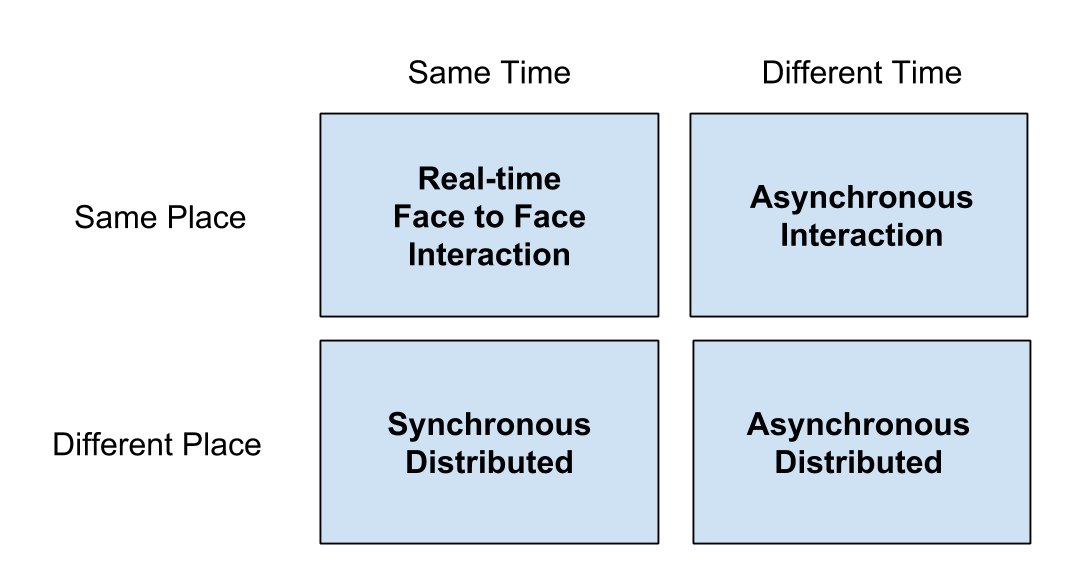
\includegraphics[width=0.8\textwidth]{assets/cscw-matrix.png}
\end{center}
\caption{Collaborative systems in time / space matrix, based on the work by Saad and Maher \cite{saad_shared_1996}.}
\label{fig:cscw-matrix}
\end{figure}


CSCW tools can also be used to create disruption to the hierarchies of the applied work environment, while getting more of the stakeholders involved in the creation of the information. For example in kindergartens the primary gatekeepers for the information flow towards children's homes are the kindergarten nurses. On a research by Näsänen et al. (2009) a web service for showing parents photos taken on the kindergarten were created. One of the goals for the research was to allow efficient way of displaying the life on the kindergarten to the children's parents, whom usually just drop off and pick up the children without being otherwise present. The children also had access to smartphones with camera, allowing them to upload photos directly to the availability of homes without the moderation of kindergarten nurses. \cite{nasanen_mobile_2009}

The real-life case study of this thesis is essentially an application which provides tools for computer supported collaborative work on kindergarten environment. Awareness of activities and events within the kindergarten are distributed to all the nurses and also to the parents if it concerns their own children. 







%% ----------------------------------
\section{Connectivity Issues}
% vai pelkkä "Internet Connectivity"?
% http://dl.acm.org/citation.cfm?id=2307649 ?
 % - eri tavat yhdistää internetiin (piuhayhteys, wlan, mobiilidata)
 % - kännyverkon toiminnasta jotain?

 % - kännyverkon toimivuuden vaihtelun yleisyydestä
 % - yleisimmät ongelmatilannetyypit


% Tänne yhdistettynä jotenkin myös vanha "existing methods to solve offline problem" -rojut:
% Minkälaisia offline ratkaisuja on olemassa web/känny-puolella (miten google/microsoft yms. ovat lähestyneet ongelmaa)?
% % onko muita kenttäkokeita tehty offline-moodiin liittyen??

For a single-page application it is possible to work without connection to the outside world, in case the application code is delivered to the device via some medium. For example to a spreadsheet application this might be a highly feasible idea. However to applications which interacts with the surrounding world some kind of connectivity is required in order to spare the person using the system having to input all the data into it. When it comes to CSCW applications, where one of the key points is the \textit{collaboration}, at least occasional Internet connectivity is mandatory. This makes issues on the Internet connectivity status and quality to concern closely CSCW applications. % HOX tää vois toisaalta olla myös ton research gapin rojua? 

On many of the scenarios and application areas where CSCW is applied using desktop computers is challenging or impossible. Often the usage is outlined to the smartphone or/and tablet usage just by the requirement of having the access to the system with the users on all occasions. If the information needs to be accessed immediately on the fly, importable devices are out of the question.

For mobile devices the medium for the ``last mile''\footnote{Metaphor used in telecommunication industry when referring to the part of the network that reaches the customer. When looking from the customer's perspective it can be named as the ``first mile.''} of connecting to the Internet is wirelessly over the radiowaves using cellular network. As more and more of the usage of the Internet moves to the mobile devices, the unprecedented cellular traffic growth can easily exceed the deployment speed of cellular infrastructures \cite{qian_web_2012}. This results in a certain \textit{guaranteed unreliability} to the connections of devices using the mobile broadband as their primary method of reaching the Internet. For the time being applications where the possibility of continuous usage is critical bracing oneself to the possible temporary Internet outages is one of the factors which must be taken into account.

One possible solution in overtaking the problems caused by the excess load of cellular networks is to use Wireless LANs as the last mile. With correct configuration this makes the wireless access as reliable as is the Internet connection of the WLAN's base station. However it is not exceptional for a CSCW system to be operated on various locations, resulting in a situation where sometimes usage of cellular network is mandatory. For applications where the SLAs\footnote{Service Level Agreement} are strict and system is used from various locations this method does not deliver any relief.

This thesis studies the issues on the Internet connectivity only from the application level, within the possibilities provided by the browser environment on handling the problem. Possible solutions available on the network-level are ignored.





%% ----------------------------------
\section{Research Gap}
% -> Gappiin ehkä jotain, että verkkovälitteistä vuorovaikutusta on tutkittu paljon (katso CSCW kamaa) ja että mobiiliverkojen tutkimus/kehitys/käyttö ollut räjähdymäistä. Kuitenkaan ei ole paljoa tutkimusta siitä kuinka verkon katkeaminen vaikuttaa reaalisaikaista tiedonvälitystä vaativan sovelluksen käyttökokemukseen ja kuinka sovellussuunnittelussa tulisi katkot ottaa huomioon. 


% This chapter focuses on the background of today's web applications and the literature that relates to the circumstances causing the connectivity issues. This chapter addresses the basics of today's web technologies and the methods that makes offline supported features possible. This chapter coverages also briefly principles on mobile device communication on the network layer, the ideology on Computer Supported Collaborative Work and takes a glimpse on already existing efforts done on solving the offline issue in web applications.  % VANHA INTRO-intro


% "Tämän dipan käsittelemä aihe sijaitsee kolmen edellisen kappaleen keskiössä -> CSCW mahdollistettuna SPA:na mutta Internet-yhteyden katkeamisten riivaamana

\begin{figure}[t]
\begin{center}
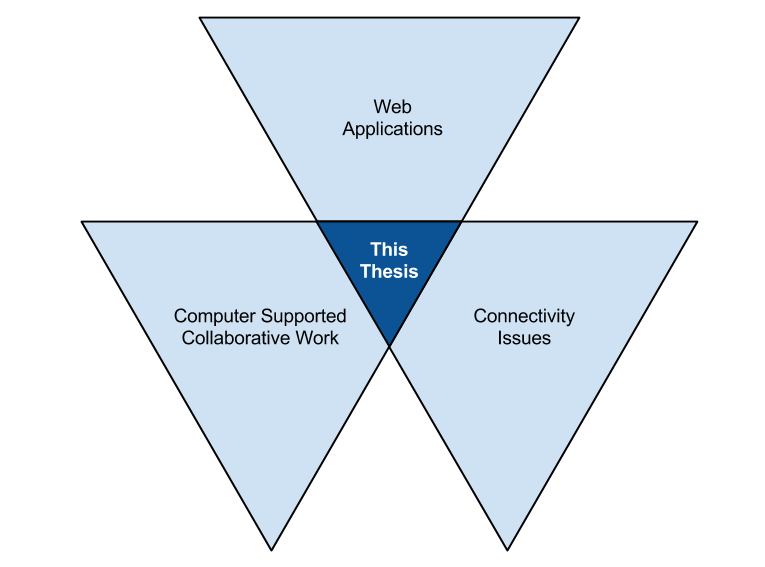
\includegraphics[width=0.8\textwidth]{assets/researchgap.png}
\end{center}
\caption{The research gap covered by this thesis}
\label{fig:researchgap}
\end{figure}

This thesis studies the overlap of the themes previously introduced in this chapter, as can be seen on the visualization in Figure~\ref{fig:researchgap}. This thesis studies what is required from a \textit{single-page application} which enables \textit{computer supported collaborative work} for the users on a environment where \textit{issues with the Internet connectivity} happens regularly. 

CSCW has been studied widely for over the past two decades. The need for streamlining working methods in favor more productivity makes efficient will make applications enabling it only more essential and common.  

The fast-paced evolution of web technologies have created a powerful platform for application development which is ubiquitously present and available everywhere. On the last decade it was available on desktop computers, today it reaches 40~\% of the Earth's population due of increasing usage of mobile devices and tablets\footnote{http://www.internetlivestats.com/internet-users/} and by 2020 \textit{4.9 billion} devices is estimated to be connected\footnote{http://www.gartner.com/newsroom/id/2905717} thanks to the \textit{Internet of Things} (IoT). This will make web technologies only more appealing method for application creation on the future.

With all this taken into account, it would not be surprising if creating applications with the web stack and the need for having an offline support on them would only get more common. Even without the rising need of these kind of applications, the user experience of any web application used over cellular network can be improved significantly with the implementation of a proper offline support, making research around it useful. On top of that there are no existing research covering all of these themes together.









% toistaiseksi hyllytetty kappale, nämä asiat tohon internet connectivity issuesiin messiin
%% ----------------------------------
% \section{Existing Solutions for the Offline Problem}
